\section{Experiments}
\label{sec:experiments}

We evaluate our proposed algorithms on real-world traces to answer three key questions: (1) What is the economic potential of optimal routing? (2) Can our online algorithms approach offline optimal under uncertainty? (3) Does latency-aware routing with hedging reduce SLO violations in production?

\subsection{Setup}

\paragraph{Datasets.} We use three real-world datasets plus one synthetic trace (Table~\ref{tab:datasets}). \textbf{ShareGPT} (201K requests) represents standard chatbot workloads. \textbf{FreeInference} (371K requests) represents diverse API gateway traffic with high variance. \textbf{Enterprise} (55K requests) is an anonymized production coding assistant with long contexts and the highest cost variance (CV $> 2$). \textbf{BurstGPT} (1.4M requests) combines BurstGPT arrival timestamps with ShareGPT prompts for online evaluation.

\begin{table}[h]
\caption{Dataset Statistics}
\label{tab:datasets}
\vskip 0.1in
\begin{center}
\begin{small}
\begin{tabular}{@{}lrrrrr@{}}
\toprule
Dataset & Reqs & Days & Models & In & Out \\
\midrule
ShareGPT & 201K & 7 & 1 & 156 & 423 \\
FreeInference & 371K & 90 & 12 & 892 & 1247 \\
Enterprise & 55K & 84 & 8 & 2341 & 3892 \\
BurstGPT & 1.4M & 61 & 1 & 234 & 512 \\
\bottomrule
\end{tabular}
\end{small}
\end{center}
\vskip -0.1in
\end{table}

\paragraph{Baselines and Pricing.} We compare against \textbf{All-API} (cost upper bound), \textbf{Greedy} (FCFS to subscription), and \textbf{Offline Optimal} (Stage 1/2 oracles). Pricing follows DeepSeek-R1: \$0.55/1M input, \$2.19/1M output tokens.

\subsection{Cost Efficiency}

\paragraph{Quota-Based Routing (Stage 1).}
With quota constraints alone, Greedy routing saves 17--81\% across datasets, while Optimal achieves 35--98\%---Greedy captures only 49--83\% of optimal savings. The gap is largest on high-variance workloads (Enterprise: CR 4.36$\times$), confirming that opportunity cost matters. Figure~\ref{fig:sensitivity} shows this gap widens with quota size: as quota increases, Optimal becomes more selective while Greedy continues wasting slots on low-value requests.

\begin{figure*}[t]
\vskip 0.1in
\begin{center}
\centerline{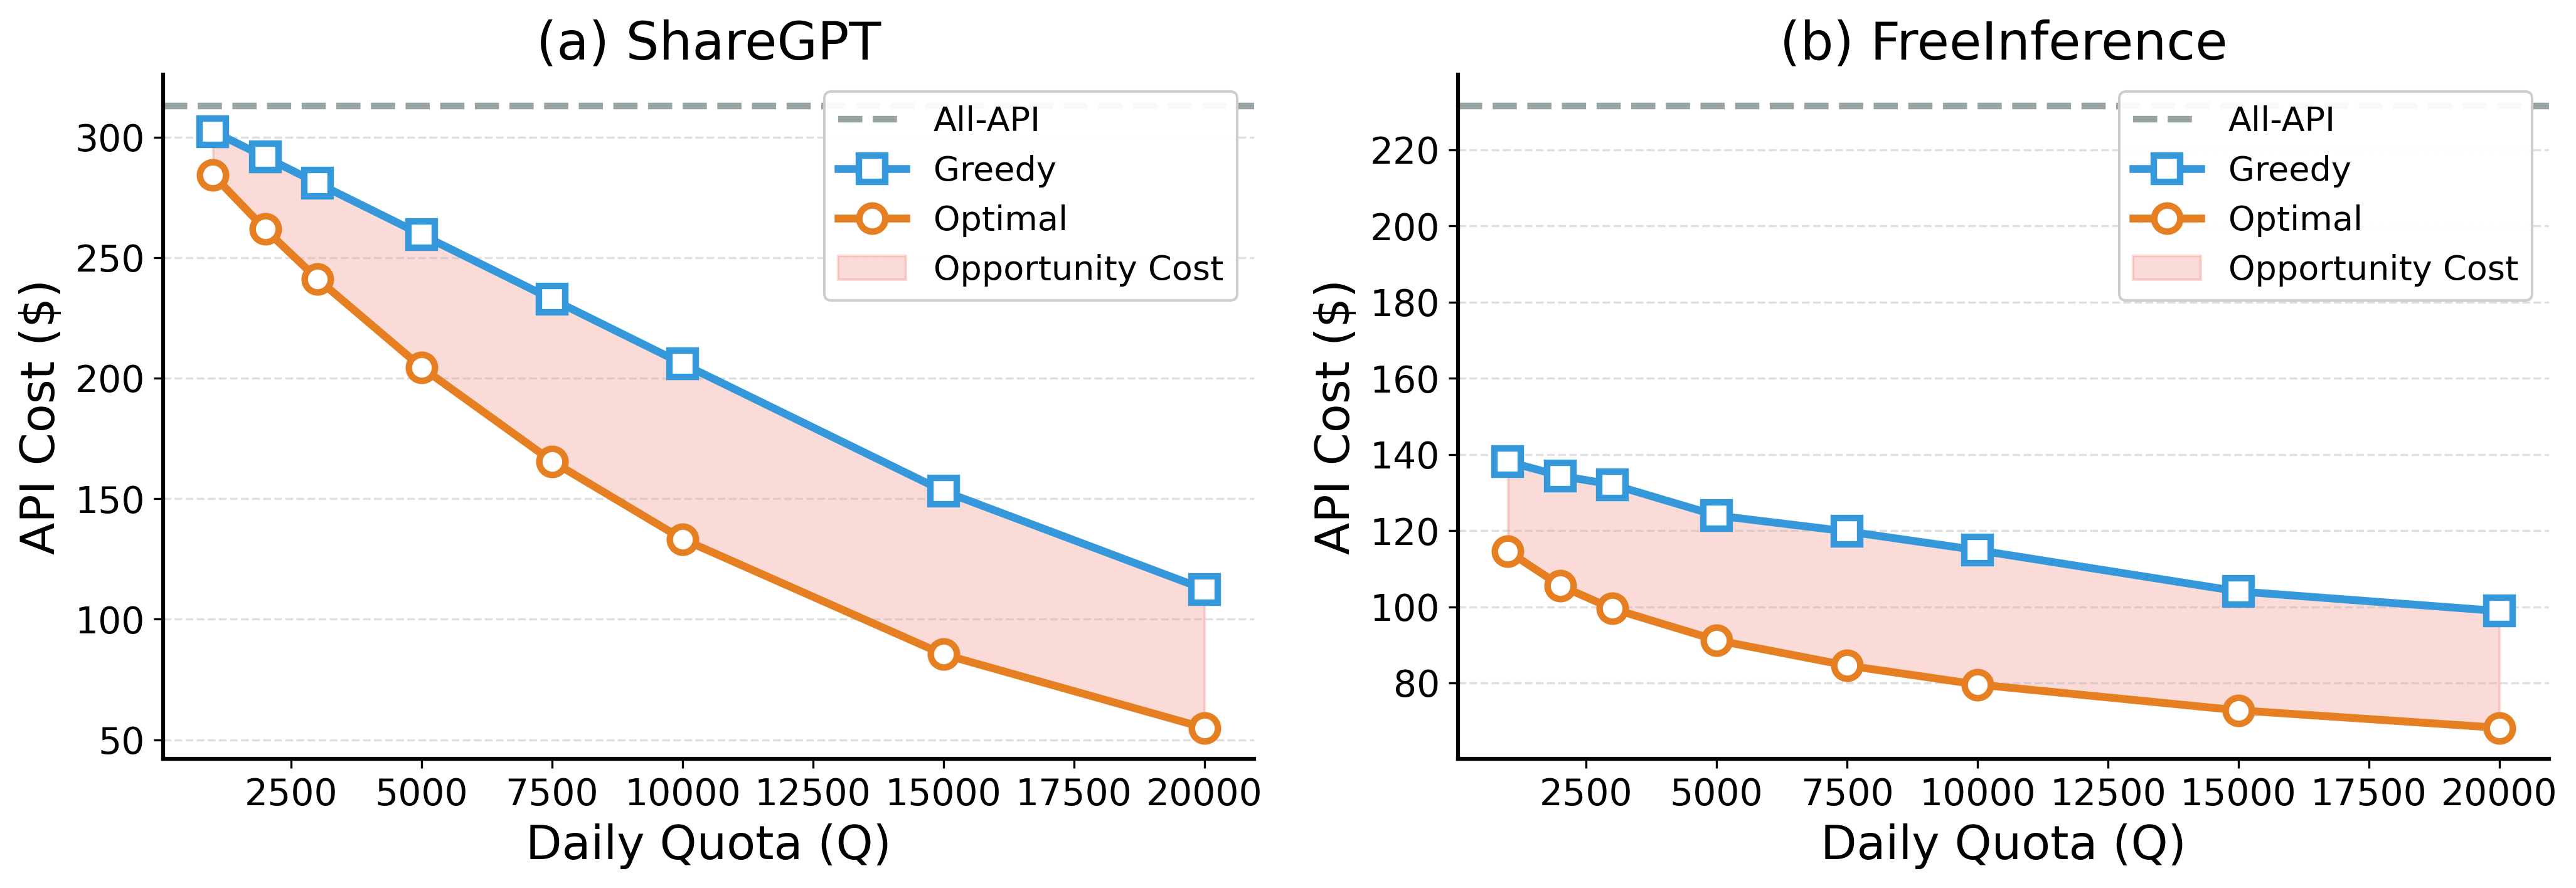
\includegraphics[width=0.95\textwidth]{images/fig2_sensitivity_combined.png}}
\caption{API cost vs quota size. The gap between Greedy and Optimal widens as quota increases, especially for multi-model workloads. The shaded area represents the opportunity cost that Greedy fails to capture.}
\label{fig:sensitivity}
\end{center}
\vskip -0.2in
\end{figure*}

\paragraph{Concurrency Constraints (Stage 2).}
For small models (e.g., Llama-3-8B), concurrency limits rarely bind before quota exhaustion. However, for larger models (70B+) with low effective concurrency ($C_{\text{eff}}=2$), physical constraints become binding (Figure~\ref{fig:concurrency_impact}). The ILP-based Stage 2 routing becomes essential.

\begin{figure}[ht]
\vskip 0.1in
\begin{center}
\centerline{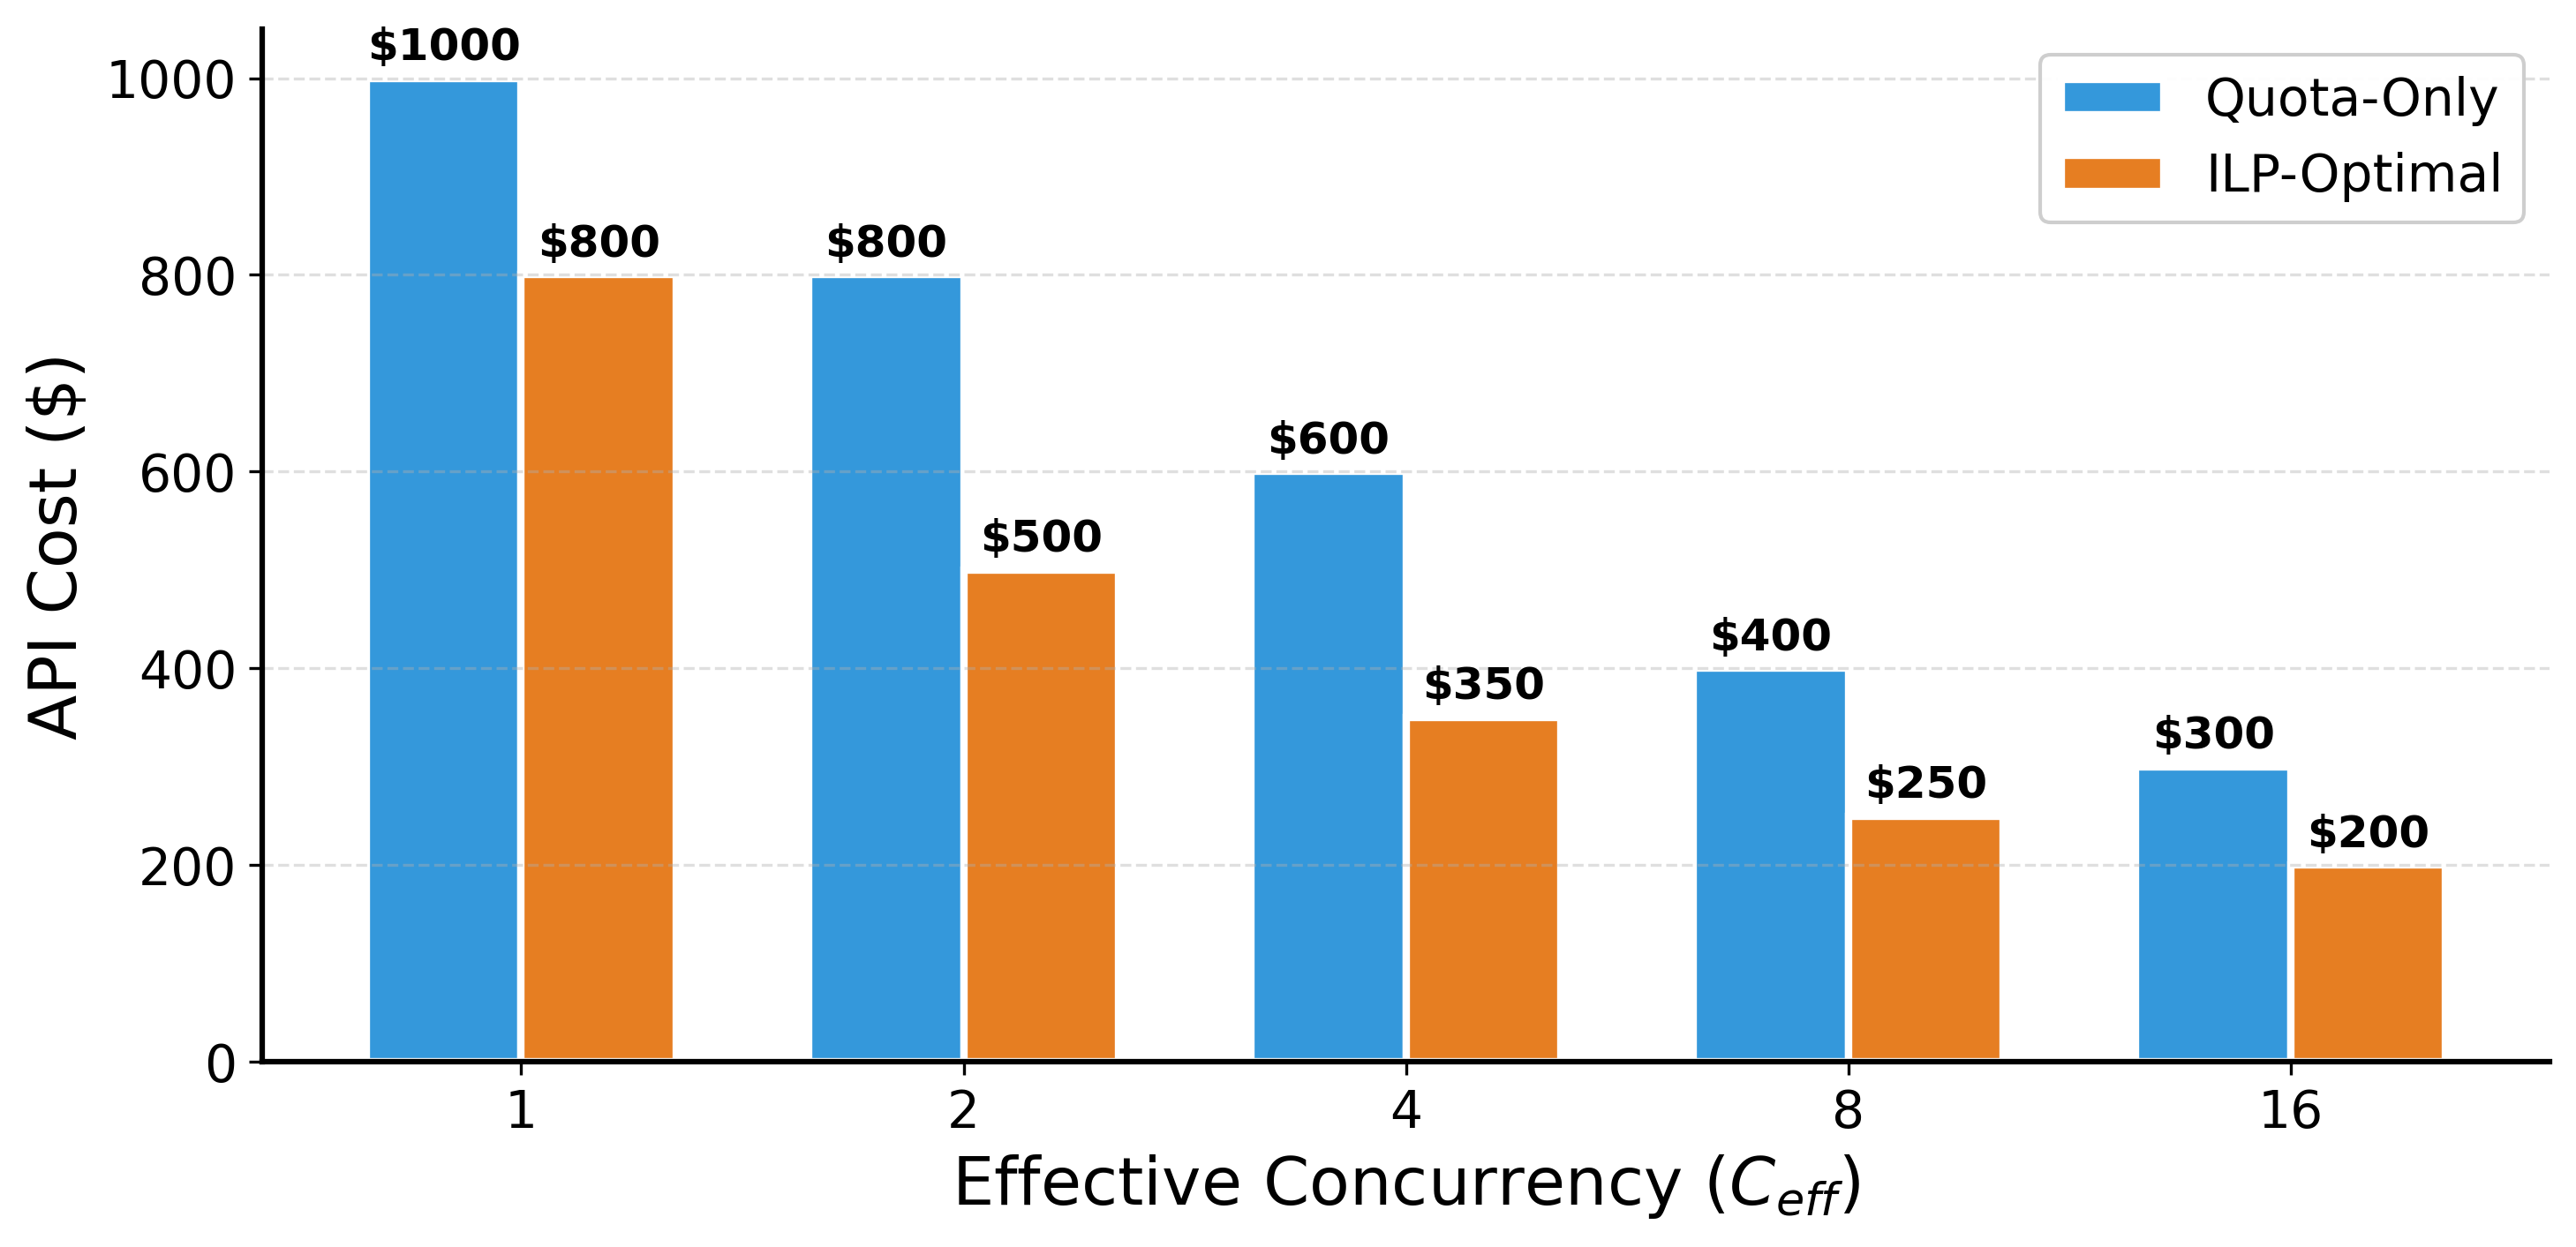
\includegraphics[width=\columnwidth]{images/single_model_comparison_rednote.png}}
\caption{Impact of model size on cost. As effective concurrency decreases, the gap between Quota-Only and ILP-Optimal widens.}
\label{fig:concurrency_impact}
\end{center}
\vskip -0.2in
\end{figure}

\paragraph{Online Joint Optimization.}
On Enterprise (54K requests, $C=8$), our PrimalDual algorithm achieves 99\% savings with CR 0.57$\times$---\textit{surpassing} the ILP-Optimal (1.0$\times$). This counterintuitive result arises because ILP discretizes time into 1-second slots, causing capacity fragmentation. PrimalDual's continuous-time event-driven admission captures opportunities that batch optimization misses. For comparison, $S_Q$-Only saves only 2\% (quota insufficient when costs vary), $S_C$-Only saves 68\% (powerful but scheduling-limited), and Greedy achieves 98\%.

\subsection{Robustness Under Uncertainty}

\paragraph{Online Performance.}
On BurstGPT (1.4M requests), our PD-EMA algorithm achieves CR 1.18$\times$, approaching the theoretical limit and outperforming Greedy (1.30$\times$). The learning-augmented variant LA-PD achieves 1.19$\times$---slightly worse than the simpler EMA approach.

\paragraph{Predictor Analysis.}
A 2$\times$2 ablation crossing predictors (EMA vs Histogram) with decision rules (Primal-Dual vs LA-PD) reveals that EMA + Primal-Dual achieves the best CR (1.18), while all other combinations achieve 1.19. Calibration analysis (Figure~\ref{fig:calibration}) explains this paradox: EMA's q50 coverage is 72\% (over-estimation), while Histogram achieves 56\% (near-ideal). Yet EMA performs better because its over-estimation naturally implements a conservative policy, and it adapts quickly to distribution shifts. For routing, \textbf{responsiveness trumps calibration}.

\begin{figure}[ht]
\vskip 0.1in
\begin{center}
\centerline{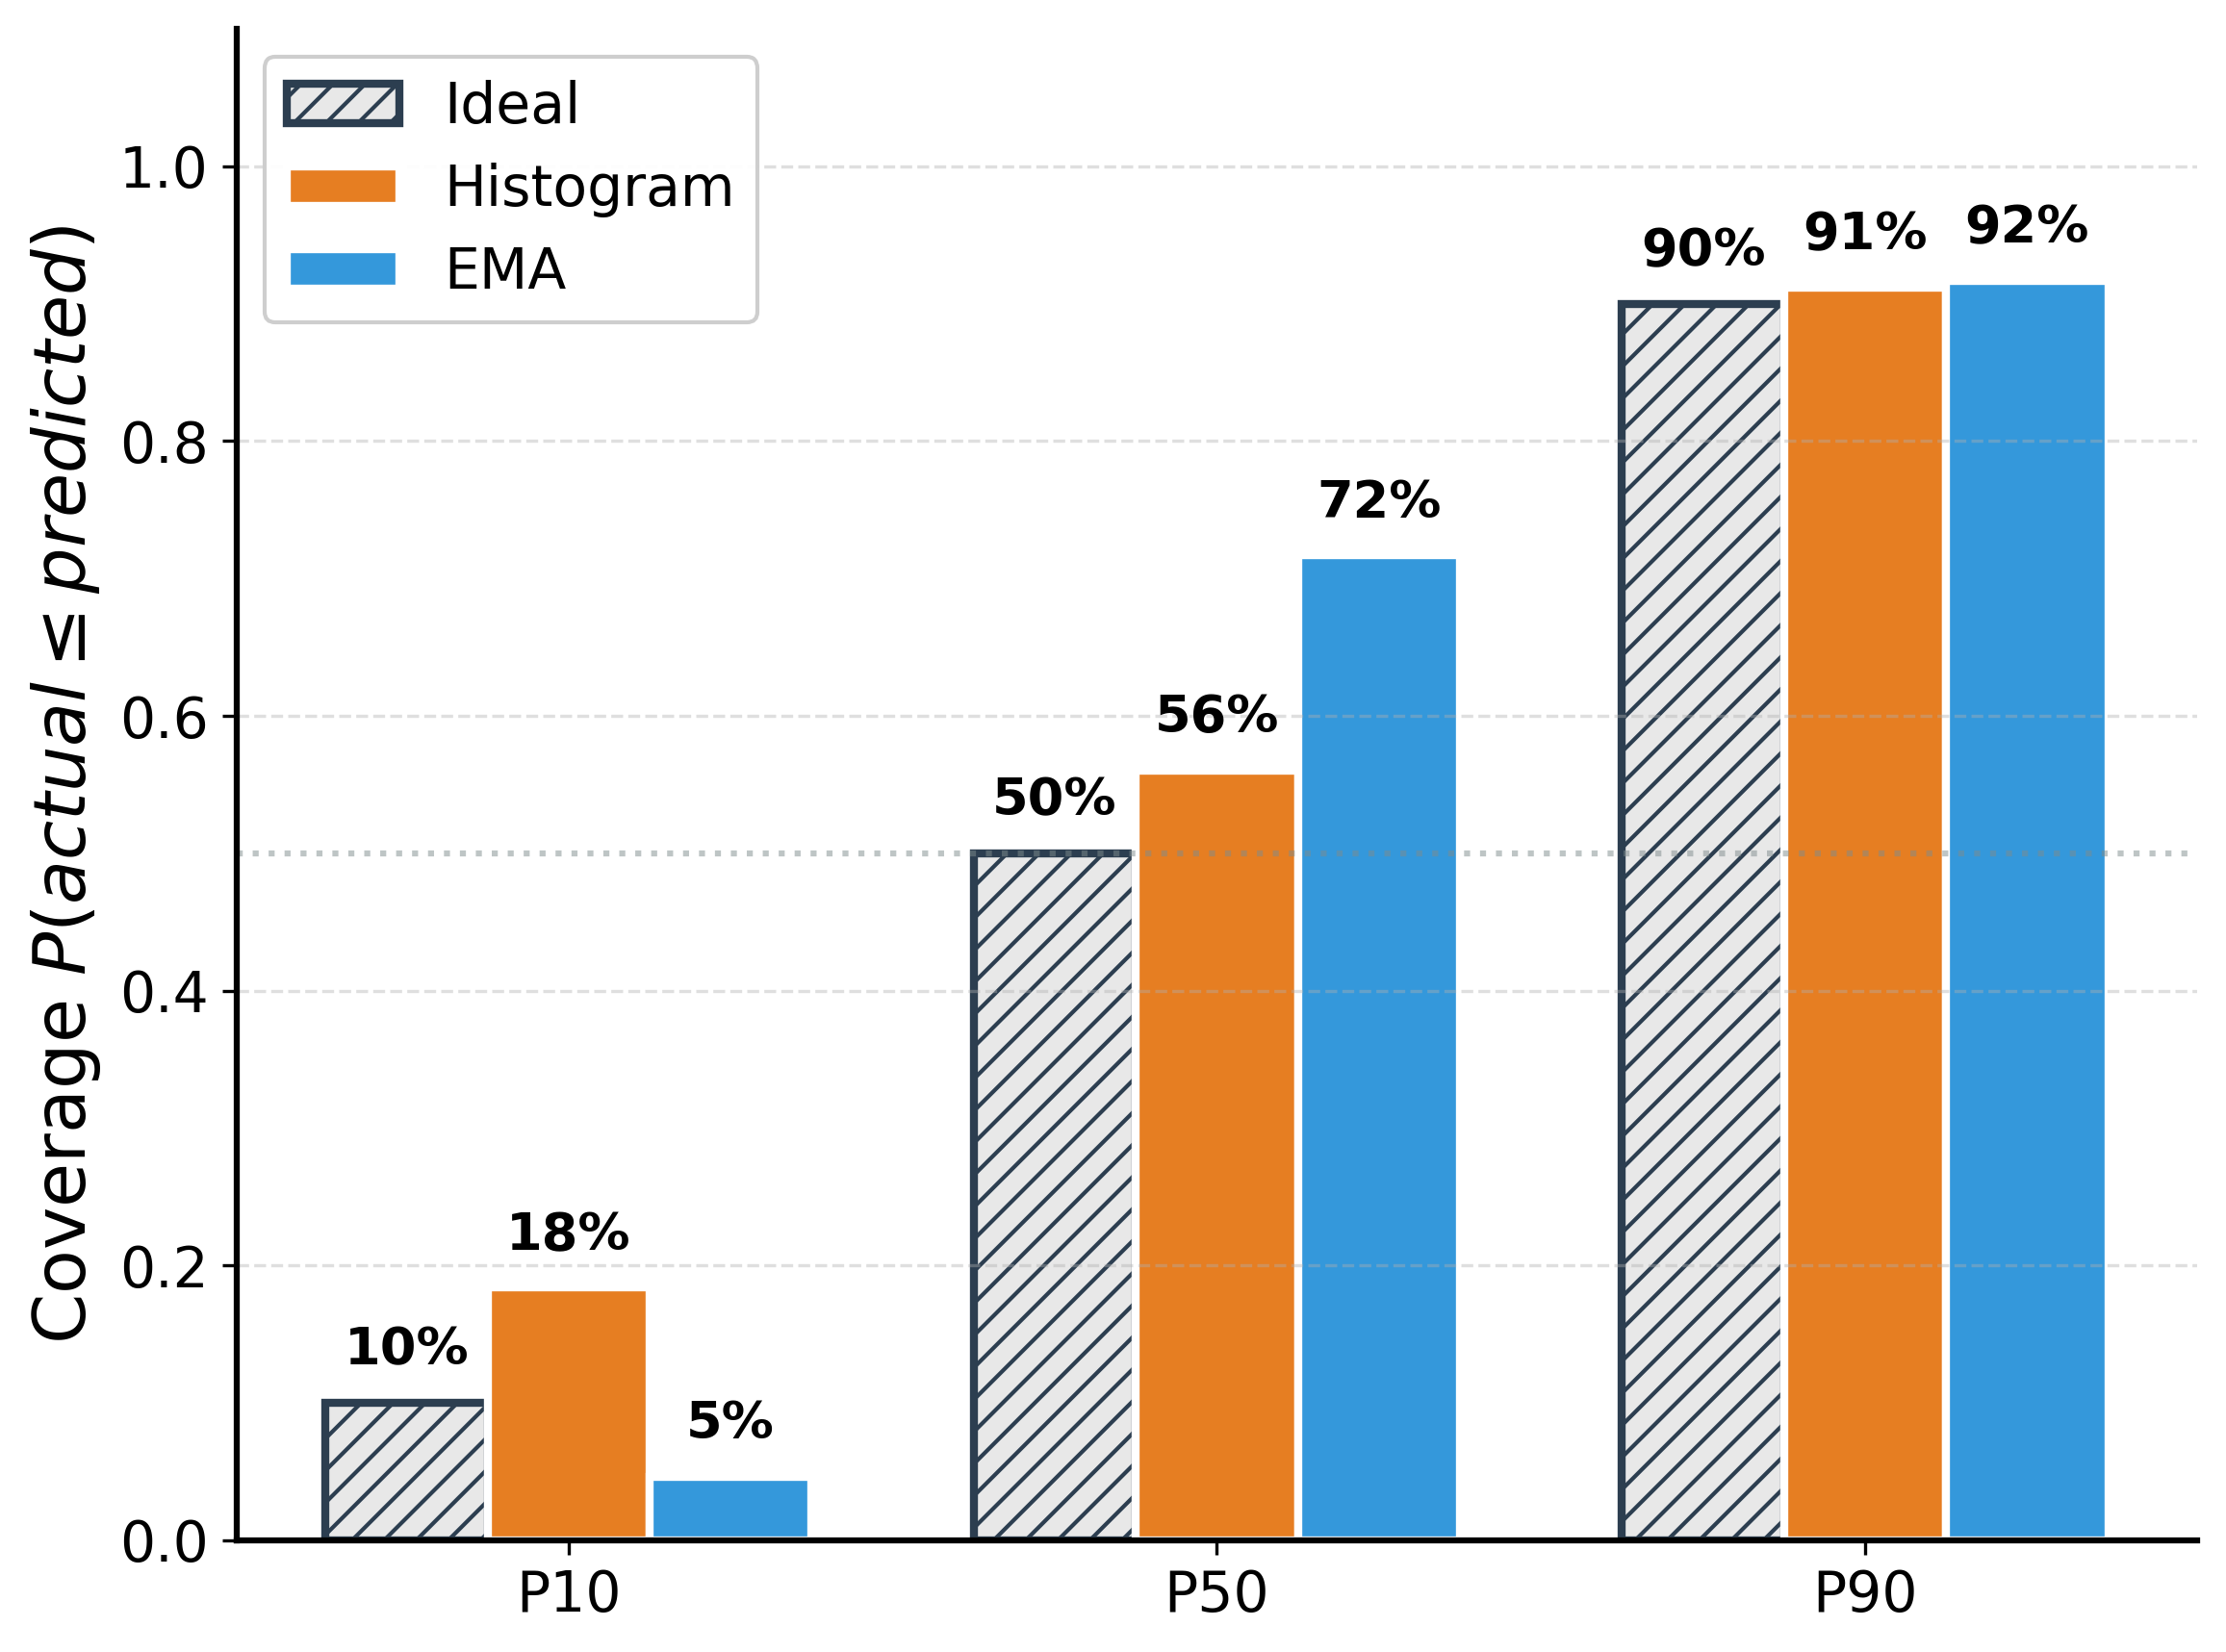
\includegraphics[width=0.85\columnwidth]{images/online_calibration.png}}
\caption{Predictor calibration. Histogram is better calibrated (closer to diagonal), but EMA achieves better routing due to faster adaptation to distribution shifts.}
\label{fig:calibration}
\end{center}
\vskip -0.2in
\end{figure}

\subsection{Latency-Aware Routing}

We evaluate latency-aware routing on OpenRouter, serving Llama-3.3-70B-Instruct across 12+ providers.

\paragraph{Provider Heterogeneity.}
Probing 12 providers over 24 hours ($n \approx 11$K samples each) reveals P99 latencies ranging from 796ms (Groq) to 16,149ms (Hyperbolic)---a 20$\times$ variation. Even providers with similar medians differ substantially in tail behavior (CV ranges 0.60--4.75), motivating online profiling over static configuration.

\paragraph{LP-Based Mixing.}
We solve for routing fractions $\pi_j$ minimizing cost subject to $\sum_j \pi_j F_j(L) \geq 0.99$ (P99 SLO at threshold $L$). At tight SLOs (2s), optimal mix favors Groq (fast, expensive); as SLO relaxes to 5s, traffic shifts to cheaper providers, reducing cost by 3$\times$ (see Figure~\ref{fig:latency_pareto} in Appendix).

\paragraph{Smart Hedging.}
To guarantee tail latency without over-provisioning, we trigger backup requests when elapsed time exceeds the primary provider's P90 threshold. Simulation shows residual-based hedging eliminates SLO violations with only 3\% cost overhead, while always-hedging costs 3.3$\times$ more.

\paragraph{Production Evaluation.}
We replay a 24-hour trace (BurstGPT timestamps + ShareGPT prompts) against the live OpenRouter API, sending each request to all policies simultaneously for fair comparison. Table~\ref{tab:openrouter_comparison} shows results.

\begin{table}[ht]
\caption{24-Hour Evaluation vs OpenRouter (SLO = 2s)}
\label{tab:openrouter_comparison}
\vskip 0.1in
\begin{center}
\begin{small}
\begin{tabular}{@{}lrrrr@{}}
\toprule
Policy & P50 & P99 & Viol. & Cost \\
\midrule
OpenRouter Auto & 820ms & 7828ms & 23.8\% & \$1.81 \\
LP-Mix & 418ms & 3659ms & 5.3\% & \$0.98 \\
Smart Hedge & 419ms & 1431ms & 0.8\% & \$1.15 \\
\bottomrule
\end{tabular}
\end{small}
\end{center}
\vskip -0.1in
\end{table}

Smart Hedge reduces SLO violations by \textbf{31$\times$} (0.8\% vs 23.8\%) and P99 latency by \textbf{5.5$\times$} (1.4s vs 7.8s) compared to OpenRouter's default routing, while saving \textbf{37\%} cost (\$1.15 vs \$1.81). Hedging triggered on 15.6\% of requests, demonstrating selective activation. LP-Mix alone achieves 46\% cost savings but higher tail latency; smart hedging trades modest cost for dramatically better latency guarantees.
